\chapter{Model order reduction for nonlinear dynamical systems}
\label{MOR_chap}
In this chapter we present two methods for model order reduction of nonlinear dynamical systems. First, we present the method of Proper Orthogonal Decomposition (POD) which constructs a matrix $U_\ell \in \mathbb{R}^{N \times \ell}$ such that the subspace $\mathcal{U}_\ell := \text{range}(U_\ell)$ is low-dimensional and a Galerkin projection of the full-order dynamical system onto $\mathcal{U}_\ell$ still captures most of the dynamical behavior of the original system. An improvement of POD that also reduces the dimension of the involved nonlinearity is given by the Discrete Empirical Interpolation Method (DEIM). We end the chapter with an application of POD-DEIM to the nonlinear Burgers' equation and present both accuracy and performance of the reduced model in comparison to the numerical solution of the full-order model. We will put a special focus on the performance benefit of POD-DEIM compared to a purely POD-reduced model.
\section{The Proper Orthogonal Decomposition (POD)}
The focus of this chapter lies on nonlinear dynamical systems of the form
\begin{align}
 \label{NonLinSys}
 \frac{d}{dt} \mathbf{y}(t) &= A \mathbf{y}(t) + \mathbf{F}(t,\mathbf{y}(t)), \quad t > 0, \\
 \label{NonLinSysIC}
 \mathbf{y}(0) &= \mathbf{y}_0,
\end{align}
which for example arise after spatial discretization of time-dependent nonlinear partial differential equations (PDEs). Therefore, we assume that the vector of unknowns $\mathbf{y}$ is of dimension $N$ and the function $\mathbf{F}:[0,T] \times \mathbb{R}^N \rightarrow \mathbb{R}^N$ captures the nonlinearity of the dynamical behavior. We have chosen the form \eqref{NonLinSys} in order to stress the difference between a linear and a nonlinear term in the dynamical behavior. We will see that a POD-reduction leads directly to a dimension reduction of the linear term while the evaluation of the nonlinear term still depends on the full dimension $N$. We will denote the dimension of the unknown vector $\mathbf{y}(t)$ with a capital $N$ in order to remind that this is the \textit{large} dimension which we seek to reduce. In the same way, we will call the (small) dimensions that are obtained by MOR techniques with small letters $\ell,m$ in order to point out that $\ell,m \ll N$.
\subsection{Optimality of the POD basis}
The overall aim of POD is the projection of the governing equations \eqref{NonLinSys}-\eqref{NonLinSysIC} onto a suitable subspace $\mathcal{U}_\ell$ of dimension $\ell \ll N$ that captures most of the dynamical behavior of the original system. In order to obtain this subspace, the so-called matrix of snapshots defined as
\begin{align}
\label{snapshots}
Y := [\mathbf{y}(t_1), \mathbf{y}(t_2), ..., \mathbf{y}(t_{n_s})] \in \mathbb{R}^{N \times n_s},
\end{align}
plays a key role. The solution vector $\mathbf{y}$ at $n_s$ different time instances form the columns of the matrix $Y$. The integer $n_s$ is called the \textit{number of snapshots} and typically, $n_s \ll N$.

In this section, we will explain how a Singular Value Decomposition (SVD) of the snapshot matrix \eqref{snapshots} can be used to obtain an optimal projection space. More specifically, we will refer to a resultfrom \cite{V11} that shows that the optimal $\ell$-dimensional projection space is given by the span of those $\ell$ singular vectors of $Y$ that correspond to the $\ell$ largest singular values. The singular value decomposition of a rectangular matrix $Y$ is given by the following well-known theorem:
\begin{theorem}
\emph{(Singular value decomposition, \cite{G96})}
\label{svdthm}
Let $Y \in \mathbb{R}^{N \times n_s}$ of rank $d$. Then there exists a decomposition of the form
\begin{align}
\label{svd}
Y = U \bbmat D & 0 \\ 0 & 0 \ebmat V^T =: U \Sigma V^T,
\end{align}
with $U \in \mathbb{R}^{N \times N}, V \in \mathbb{R}^{n_s \times n_s}$ orthogonal and $D = diag(\sigma_1,...,\sigma_d) \in \mathbb{R}_+^{d \times d}$. The columns in $U = [\mathbf{u}_1,...,\mathbf{u}_N]$ are called the (left) singular vectors of $Y$ and for the singular values $\sigma_i$ it holds: $\sigma_1 \geq \sigma_2 \geq ... \geq \sigma_d > 0$.
\end{theorem}
\begin{proof}
Can, for example, be found in \cite[Theorem 2.5.2]{G96}.
\end{proof}
Note that due to the SVD, the following diagonalization holds
\begin{align}
\label{SVDalsEW}
Y Y^T = (U \Sigma V^T) (U \Sigma V^T)^T = U \Sigma^2 U^T,
\end{align}
and, hence, the columns of $U$ are eigenvectors of the matrix $Y Y^T$ with corresponding eigenvalues $\lambda_i = \sigma_i^2 > 0, \ i=1,...,d$.

We will next consider the optimization problem \eqref{optBasis} whose solution gives rise to the practical computation of the POD basis. We seek for an orthonormal basis $\varphi_1,...,\varphi_\ell$ such that the components of the snapshots $\mathbf{y}(t_1),...,\mathbf{y}(t_{n_s})$ are maximized when expressed in this basis. Therefore, it is desired to find the basis $\varphi_1,...,\varphi_\ell$ and the following theorem states that the left singular vectors of $Y$ solve the optimization problem \eqref{optBasis}.
\begin{theorem}
\emph{(POD basis, \cite{V11})}
\label{podthm}
Let $Y \in \mathbb{R}^{N \times n_s}$ be the snapshot matrix \eqref{snapshots} with rank $d \leq \min \{N,n_s\}$. Further, let $Y = U \Sigma V^T$ be the singular value decomposition of $Y$ with orthogonal matrices $U = [\mathbf{u}_1,...,\mathbf{u}_N]$ and $V = [\mathbf{v}_1,...,\mathbf{v}_{n_s}]$ as in \eqref{svd}. Then, for any $\ell \in \{1,...,d\}$ the solution to the optimization problem
\begin{align}
\label{optBasis}
\max_{\varphi_1,...,\varphi_\ell} \sum_{i=1}^\ell \sum_{j=1}^{n_s} |\langle \mathbf{y}_j , \varphi_i \rangle|^2 \quad s.t. \quad \langle \varphi_i,\varphi_j\rangle = \delta_{i,j} \ \text{for } 1 \leq i,j \leq \ell
\end{align}
is given by the left singular vectors $\{ \mathbf{u}_i \}_{i=1}^\ell$. The vectors $\varphi_1,...,\varphi_\ell$ are called the POD basis of rank $\ell$. Here, $\delta_{i,j}$ denotes the Kronecker delta.
\end{theorem}
\begin{proof}
The proof is given in \cite[p. 5-6]{V11}
\end{proof}

%\begin{proof}
%The following proof is based on the ideas of \cite{V11}. Since \eqref{optBasis} is an equality constrained optimization problem, we consider the corresponding Lagrangian function
%\begin{align*}
%&\mathcal{L} : \mathbb{R}^N \times ... \times \mathbb{R}^N \times \mathbb{R}^{\ell \times \ell} \rightarrow \mathbb{R}\\
%&\mathcal{L}(\varphi_1,...,\varphi_\ell,\Lambda) = \sum_{i=1}^\ell \sum_{j=1}^{n_s} |\langle \mathbf{y}_j , \varphi_i \rangle|^2 + \sum_{i,j=1}^\ell \lambda_{ij} (\delta_{ij}-\langle \varphi_i,\varphi_j\rangle),
%\end{align*}
%where $\Lambda := (\lambda_{i,j})_{i,j=1}^\ell$. The first-order necessary optimality conditions of \eqref{optBasis} are then given by
%\begin{align*}
%\frac{\partial \mathcal{L}}{\partial \varphi_k}(\varphi_1,...,\varphi_\ell,\Lambda) &= 0, \quad \text{for } k \in \{1,...,\ell\}, \\
%\frac{\partial \mathcal{L}}{\partial \lambda_{i,j}}(\varphi_1,...,\varphi_\ell,\Lambda) &= 0, \quad \text{for } i,j \in \{1,...,\ell\},
%\end{align*}
%where the latter equation is equivalent to the constraint $\langle \varphi_i,\varphi_j\rangle = \delta_{i,j}$. In \cite[p. 5]{V11}, it is shown that the first condition leads to
%\begin{align}
%\label{zwschritt}
%Y Y^T \varphi_k = \frac{1}{2} \sum_{i=1}^\ell (\lambda_{i,k} + \lambda_{k,i}) \varphi_i, \quad \text{for all } k \in \{1,...,\ell\}.
%\end{align}
%The actual proof that the optimal vectors $\varphi_1,...,\varphi_\ell$ are given by the first $\ell$ left singular vectors of $Y$ is done by induction on $\ell$. First, let $\ell=1$. From \eqref{zwschritt}, it follows that $k=1$ and we get:
%\begin{align*}
%Y Y^T \varphi_1 = \lambda_{1,1} \varphi_1.
%\end{align*}
%From \eqref{SVDalsEW}, we have that this eigenequation can be expressed as an SVD with $\varphi_1$ being the first left singular vector of $Y$.
%
%Next, consider the case $\ell \geq 1$ and suppose
%\begin{align*}
%Y Y^T \varphi_k = \lambda_{k,k} \varphi_k, \quad \text{for all } k \in \{1,...,\ell\}.
%\end{align*}
%We want to show that the first-order necessary optimality conditions for a POD-basis of rank $\ell+1$ are given by
%\begin{align*}
%Y Y^T \varphi_k = \lambda_{k,k} \varphi_k, \quad \text{for all } k \in \{1,...,\ell+1\},
%\end{align*}
%and can, thus, be computed by an SVD of $Y$. Using the induction hypothesis, we only have to show that
%\begin{align*}
%Y Y^T \varphi_{\ell+1} = \lambda_{\ell+1,\ell+1} \varphi_{\ell+1}.
%\end{align*}
%Since $\{\varphi_i\}_{i=1}^{\ell+1}$ is a POD-basis, it holds that $\langle \varphi_{\ell+1},\varphi_i \rangle = 0$ for $1 \leq i \leq \ell$ and we get
%\begin{align*}
%0 &= \lambda_{i,i} \langle \varphi_{\ell+1},\varphi_i \rangle = \langle \varphi_{\ell+1}, Y Y^T \varphi_i \rangle = \langle Y Y^T  \varphi_{\ell+1}, \varphi_i \rangle \\
% &= \frac{1}{2} \sum_{j=1}^{\ell+1} (\lambda_{j,\ell+1} + \lambda_{\ell+1,j}) \langle \varphi_j,\varphi_i \rangle = (\lambda_{i,\ell+1} + \lambda_{\ell+1,i}) \quad \Rightarrow \quad \lambda_{\ell+1,i} = - \lambda_{i,\ell+1}, \ i \in \{1,...,\ell\},
%\end{align*}
%where the symmetry of $Y Y^T$ guarantees the matrix to be self-adjoint in $\langle \cdot, \cdot \rangle_{\mathbb{R}^N}$.
%
%Inserting the last relation into \eqref{zwschritt}, we obtain
%\begin{align*}
%Y Y^T \varphi_{\ell+1} &= \frac{1}{2} \sum_{i=1}^{\ell+1} (\lambda_{i,\ell+1}+\lambda_{\ell+1,i}) \varphi_{i} = \frac{1}{2} \sum_{i=1}^{\ell} (\lambda_{i,\ell+1}+\lambda_{\ell+1,i}) \varphi_{i} + \lambda_{\ell+1,\ell+1} \varphi_{\ell+1} \\
% &= \frac{1}{2} \sum_{i=1}^{\ell} \underbrace{(\lambda_{i,\ell+1}-\lambda_{i,\ell+1})}_{=0} \varphi_{i} + \lambda_{\ell+1,\ell+1} \varphi_{\ell+1} = \lambda_{\ell+1,\ell+1} \varphi_{\ell+1}
%\end{align*}
%
%We have shown that the first-order optimality conditions corresponding to \eqref{optBasis} are given by the $N \times N$ eigenvalue problems
%\begin{align*}
%Y Y^T \mathbf{u}_i = \lambda_i \mathbf{u}_i, \quad i = 1,...,\ell,
%\end{align*}
%where the vectors $\{\mathbf{u}_i\}_{i=1}^\ell$ are given by the left singular vectors of $Y$ due to \eqref{SVDalsEW}. The proof that $\{\mathbf{u}_i\}_{i=1}^\ell$ are a solution of \eqref{optBasis} can be found in \cite{V11}.
%\end{proof}
Note that this result is crucial for the practical usage of the POD method since it presents a simple way how to compute the POD basis from the snapshot matrix. The optimal projection space it then given by $\mathcal{U}_\ell = span \{\mathbf{u}_1,...,\mathbf{u}_\ell\}$. The choice of the dimension $\ell$ of the POD basis is important for the quality of the approximation of the POD model. According to \cite{V11}, there exists no theoretical bound for the approximation error depending on $\ell$. Therefore, in practice the choice of $\ell$ has to be obtained heuristically. The ratio,
\begin{align}
\label{heuristics}
\varepsilon(\ell) := \frac{\sum_{i=1}^\ell \sigma_i^2}{\sum_{i=1}^N \sigma_i^2}, \quad 1 \leq \ell \leq N,
\end{align}
 gives a good estimate of the relationship between the energy of the reduced system and the total energy. Note that $\varepsilon(\cdot)$ as a function of $\ell$ is growing fast when the considered dynamical system is suitable for model order reduction, i.e. the first singular values are large compared to the sum of all singular values. For instance, in the setting of Section \ref{BurgersPODDEIM} we present the distribution of the singular values for $\nu = 0.01$ in Figure \ref{singVal}. The numerical solution of the full-order model required a spatial discretization of $N = 80$ and a POD dimension of $\ell = 9$ already leads to $\varepsilon(9) = 0.98$ which seems to indicate that most of the dynamical behavior of the full-order system can be captured by a POD reduced model of dimension $9$. This can also be seen in Figure \ref{PODplot}.
\subsection{The projected reduced-order model}
In the previous section, we have shown that the optimal subspace $\mathcal{U}_\ell$ that captures most of the dynamical behavior of the original dynamical system is given by $\mathcal{U}_\ell = span \{\mathbf{u}_1,...,\mathbf{u}_\ell\}$, where $\{\mathbf{u}_i\}_{i=1}^\ell$ form a POD basis of dimension $\ell$. In order to construct the POD reduced-order model, we define the matrix $U_\ell := [\mathbf{u}_1,...,\mathbf{u}_\ell]$. Then, we can construct an approximation of the solution vector $\mathbf{y}$ in $\mathcal{U}_\ell$ as:
\begin{align*}
\mathbf{y}(t) \approx U_\ell \mathbf{\tilde y}(t), \quad \mathbf{\tilde y}(t) \in \mathbb{R}^\ell.
\end{align*}
A reduced-order model for \eqref{NonLinSys}-\eqref{NonLinSysIC} in terms of $\mathbf{\tilde y}(t)$ can be derived by a Galerkin projection of \eqref{NonLinSys} onto $\mathcal{U}_\ell$,
\begin{align}
\label{GalProj}
\frac{d}{dt} \mathbf{\tilde y}(t) &= U_\ell^T A U_\ell \mathbf{\tilde y}(t) + U_\ell^T \mathbf{F}(t,U_\ell\mathbf{\tilde y}(t)) \nonumber \\
 &=: \tilde A \mathbf{\tilde y}(t) + \mathbf{\tilde N}(\mathbf{\tilde y},t),
\end{align}
with $\tilde A := U_\ell^T A U_\ell \in \mathbb{R}^{\ell \times \ell}$ and nonlinearity $\mathbf{\tilde N}(\mathbf{\tilde y},t) : = U_\ell^T \mathbf{F}(t,U_\ell\mathbf{\tilde y}(t))$.

The corresponding initial condition is given by
\begin{align*}
\mathbf{\tilde y}(0) = U_\ell^T \mathbf{y}_0.
\end{align*}

We will refer to \eqref{GalProj} as the POD-reduced model. Note that the linear part of the dynamical system in \eqref{GalProj} is represented by the matrix $\tilde A \in \mathbb{R}^{\ell \times \ell}$. We see that the linear term is already independent of the full-order dimension $N$.
\section{The Discrete Empirical Interpolation Method (DEIM)}
\label{Deim_chap}
In the previous sections, we used the POD-Galerkin approach \eqref{GalProj} to construct a reduced-order model forthe full order dynamical system \eqref{NonLinSys}-\eqref{NonLinSysIC}. The system \eqref{GalProj} is of (small) dimension $\ell$ and the unknown $\mathbf{\tilde y}$ is an $\ell$-dimensional approximation of $\mathbf{y}$. However, the evaluation of the nonlinear term $\mathbf{\tilde N}(\mathbf{\tilde y},t)$ still has computational complexity that depends on the original problem size $N$ as the following shows:
\begin{align*}
\mathbf{\tilde N}(\mathbf{\tilde y},t) = \underbrace{U_\ell^T}_{\ell \times N} \underbrace{\mathbf{F}(U_\ell\mathbf{\tilde y}(t))}_{N \times 1}.
\end{align*}
The DEIM method \cite{DEIM} is an efficient way to overcome this dependence on $N$ and is, therefore, considered as an improvement of the POD algorithm. To simplifynotation, let us denote from now on $\mathbf{f}(t) := \mathbf{F}(U_\ell\mathbf{\tilde y}(t))$. We are looking for a low-dimensional approximation:
\begin{align*}
\mathbf{f}(t) \approx W \mathbf{c}(t),
\end{align*}
where $W := [\mathbf{w}_1,...,\mathbf{w}_m] \in \mathbb{R}^{N \times m}$ and the coefficient vector $\mathbf{c}(t) \in \mathbb{R}^m$, as in the POD approach. Indeed, in DEIM the projection space $span \{\mathbf{w}_1,...,\mathbf{w}_m\}$ is obtained by an SVD of the snapshot matrix of the nonlinearity
\begin{align}
\label{snapshotF}
F := [\mathbf{f}(t_1), \mathbf{f}(t_2), ..., \mathbf{f}(t_{n_s})] \in \mathbb{R}^{N \times n_s}.
\end{align}
Since $\mathbf{f}(t) = W \mathbf{c}(t)$ is an overdetermined linear system of equations in $\mathbf{c}(t)$, we select $m$ distinguished rows from both sides of the system. Therefore, we define the matrix $\mathcal{P} = [\mathbf{e}_{\wp_1},...,\mathbf{e}_{\wp_m}] \in \mathbb{R}^{N \times m}$ with $\mathbf{e}_{\wp_i} = [0,...,0,1,0,...,0] \in \mathbb{R}^N$ having its non-zero entry at the $\wp_i$-th component. If $\mathcal{P}^T W$ is nonsingular, the coefficient vector $\mathbf{c}(t)$ can uniquely be determined from:
\begin{align*}
\mathcal{P}^T \mathbf{f}(t) = (\mathcal{P}^T W) \mathbf{c}(t),
\end{align*}
and we derive an approximation of $\mathbf{f}(t)$ as:
\begin{align}
\label{approxF}
\mathbf{f}(t) \approx W \mathbf{c}(t) = W (\mathcal{P}^T W)^{-1} \mathcal{P}^T \mathbf{f}(t) =: \mathbf{\hat f}(t).
\end{align}
Note that the matrix-vector multiplication $\mathcal{P}^T \mathbf{f}(t)$ is never computed in the standard way since this would imply a dependence of the computational complexity on $N$ because $\mathbf{f}(t)$ is an $N$-dimensional vector. Instead, a left multiplication with $\mathcal{P}^T$ is by construction equivalent to the selection of $m$ entries of the vector $\mathbf{f}(t)$ which is an $\mathcal{O}(m)$ operation.

The nonlinear term in \eqref{GalProj} can, thus, be computed via
\begin{align*}
\mathbf{\tilde N}(\mathbf{\tilde y},t) &\approx U_\ell^T W (\mathcal{P}^T W)^{-1} \mathcal{P}^T \mathbf{F}(U_\ell \mathbf{\tilde y}(t))\\
&\stackrel{(\ast)}{=}\underbrace{U_\ell^T W (\mathcal{P}^T W)^{-1}}_{\ell \times m} \underbrace{\mathbf{F}(\mathcal{P}^T U_\ell \mathbf{\tilde y}(t))}_{m \times 1},
\end{align*}
where we have assumed that the function $\mathbf{F}(\cdot)$ only acts pointwise on its input vector. Hence, it is possible in step $(\ast)$ to first select the $m$ components of the input vector and then evaluate the function $\mathbf{F}$. The resulting approximation of $\mathbf{\tilde N}(\mathbf{\tilde y},t)$ does not depend on the dimension $N$ of the full order system and, moreover, we note that the matrix $U_\ell^T W (\mathcal{P}^T W)^{-1}$ does not depend on time and can, thus, be pre-computed. Note that DEIM can also be applied to general nonlinear functions that are not pointwise. We refer the reader to \cite{DEIM} for more details.

It remains to describe how the $m$ entries of $\mathbf{f}(t)$ are selected in DEIM such that the approximation $\mathbf{\hat f}(t)$ in formula \eqref{approxF} is optimal. An algorithm that successively constructs the matrix $\mathcal{P}$ for a given input basis $\mathbf{w}_1,...,\mathbf{w}_m$ is proposed in \cite[Section 3.1]{DEIM} and presented here as Algorithm \ref{alg:DEIM}. In the initialization step, the first index $\wp_1 \in \{1,...,N\}$ is selected corresponding to the largest components in magnitude of the first input basis vector $\mathbf{w}_1$. The loop over $i=2$ to $i=m$ selects the indices corresponding to the largest component of the residual $\mathbf{r}$ between the input basis $\mathbf{w}_i$ and its approximation within the subspace $span \{\mathbf{w}_1,...,\mathbf{w}_{i-1}\}$.
\begin{algorithm}[H]
\caption{The DEIM algorithm, \cite{DEIM}}
\label{alg:DEIM}
\begin{algorithmic}[1]
\STATE \textbf{INPUT: } $\{\mathbf{w}_i\}_{i=1}^m \subset \mathbb{R}^N$  linear independent
\STATE \textbf{OUTPUT: } $\vec \wp = [\wp_1,...,\wp_m]^T \in \mathbb{R}^m, \ \mathcal{P} \in \mathbb{R}^{N \times m}$
\STATE $[|\rho|,\wp_1] = \max \{|\mathbf{w}_1|\}$
\STATE $W = [\mathbf{w}_1], \mathcal{P} = [\mathbf{e}_{\wp_1}], \vec \wp = [\wp_1]$
\FOR{$i = 2$ to $m$}
\STATE Solve $(\mathcal{P}^T W) \mathbf{c} = \mathcal{P}^T \mathbf{w}_i$ for $\mathbf{c}$
\STATE $\mathbf{r} = \mathbf{w}_i - W \mathbf{c}$
\STATE $[|\rho|,\wp_i] = \max \{|\mathbf{r}|\}$
\STATE $W \leftarrow [W \ \mathbf{w}_i], \mathcal{P} \leftarrow [\mathcal{P} \ \mathbf{e}_{\wp_i}], \vec \wp \leftarrow \begin{bmatrix} \vec \wp \\ \wp_i \end{bmatrix}$
\ENDFOR
\end{algorithmic}
\end{algorithm}
An illustrative example taken from \cite{DEIM} is given by the nonlinear parameterized function:
\begin{align}
\label{1Dex}
s(x,\mu) = (1-x) \cos(3 \pi \mu (x+1)) e^{-(1+x)\mu}, \quad x \in [-1,1], \mu \in [1,\pi],
\end{align}
to which the DEIM algorithm was applied based on $100$ equidistantly spaced points $x_i \in [-1,1]$ and $51$ snapshots for $\mu_j \in [1,\pi]$. Figure \ref{DeimPointsa} shows that the first DEIM indices obtained by Algorithm \ref{alg:DEIM} are chosen in a region where most of the dynamics of $s$ occurs. In Figure \ref{DeimPointsb}, it can be seen that for $\mu = 3.1$, the approximation $\hat s$ based on DEIM with dimension $m=10$ gives a good result compared to the $100$-dimensional original model.
\begin{figure}[H]
\centering
\subfloat[First six POD bases with DEIM points.]{\label{DeimPointsa}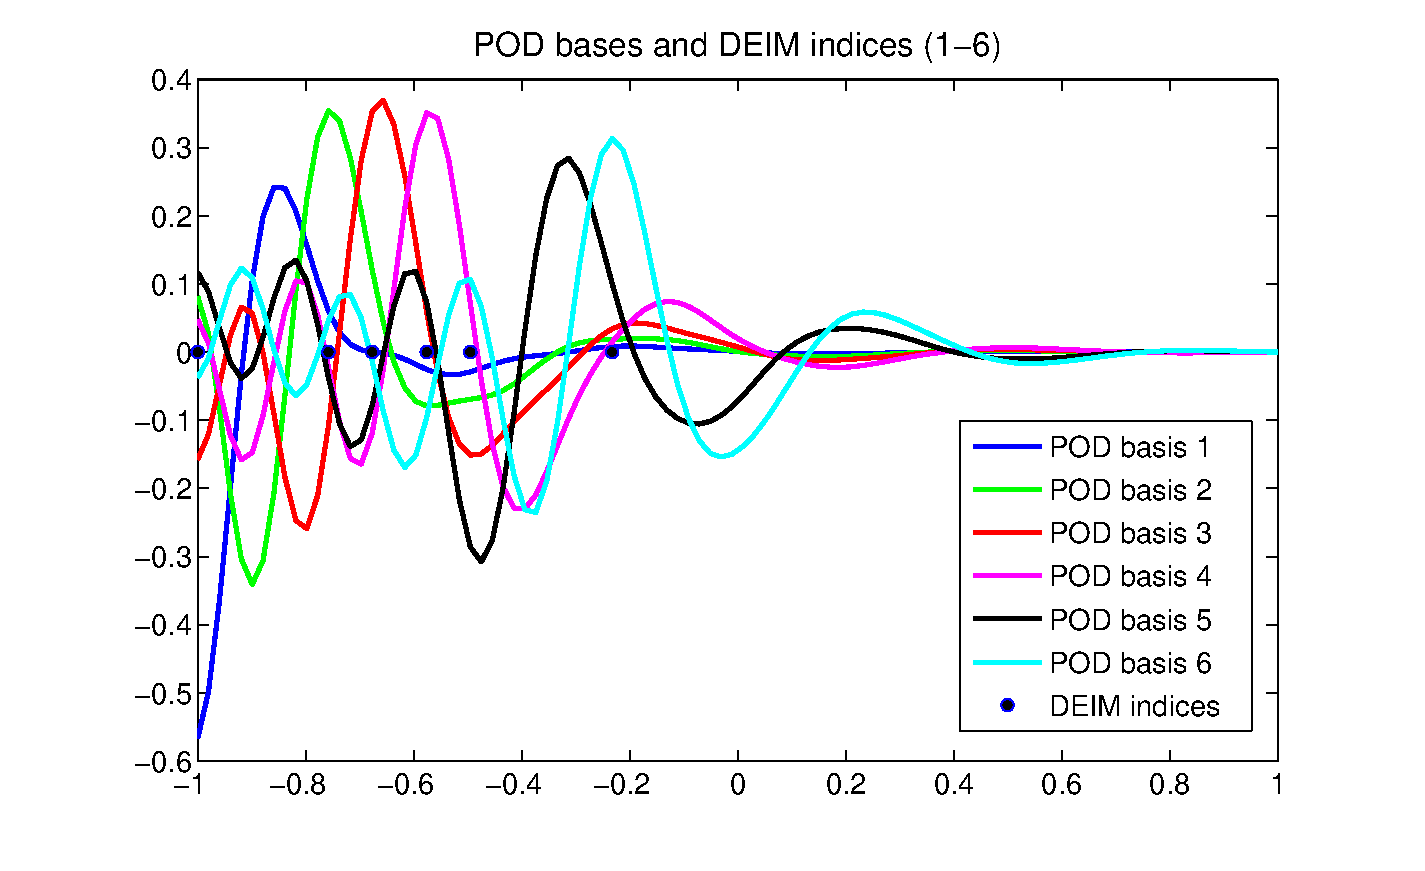
\includegraphics[width=0.49\textwidth]{plots/DeimPoints}}\hfill
\subfloat[DEIM approximation of dimension $10$.]{\label{DeimPointsb}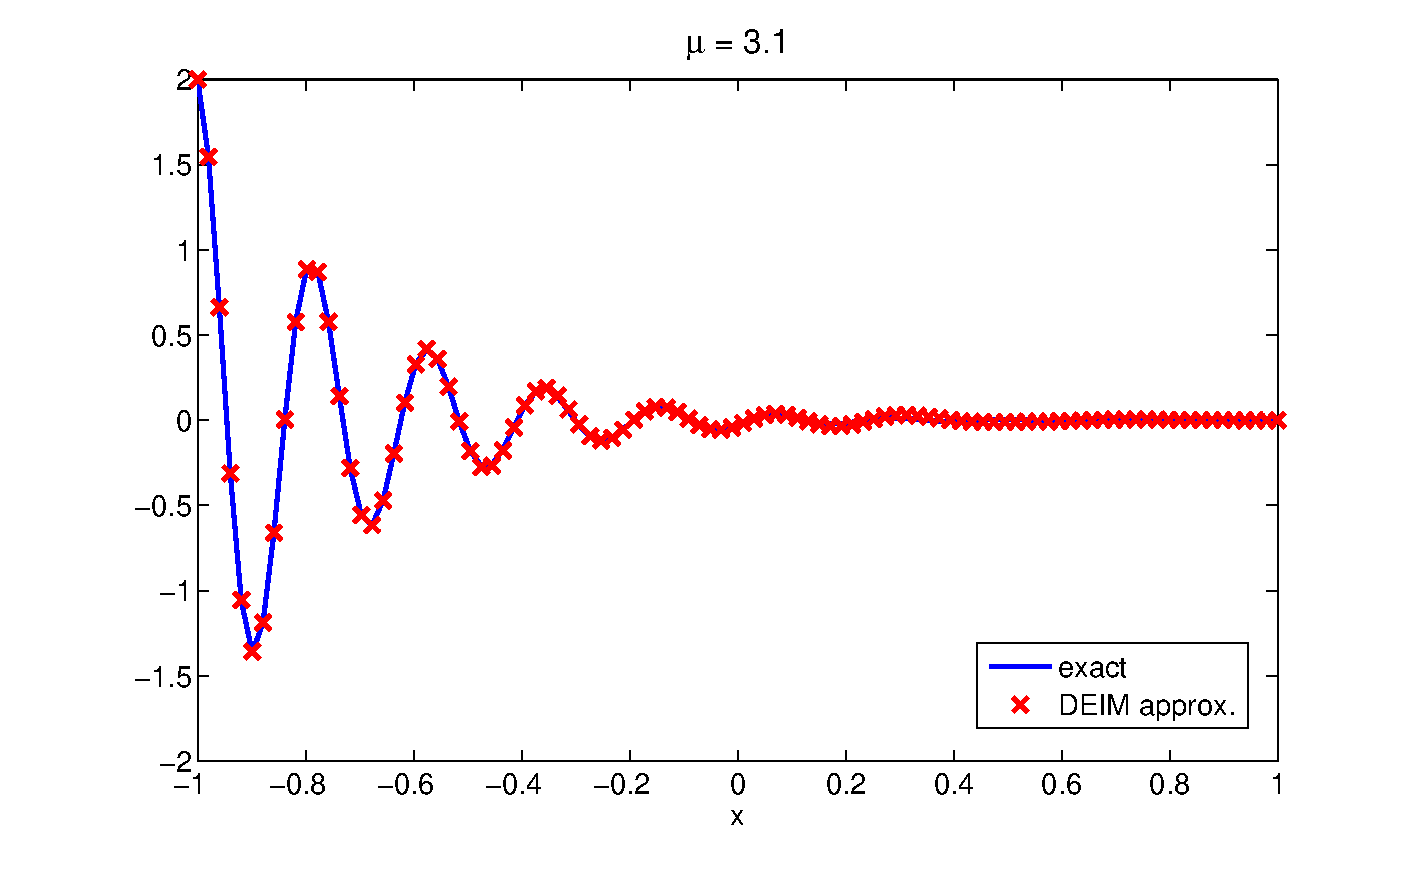
\includegraphics[width=0.49\textwidth]{plots/DeimApprox1D}}
\caption{The location of the DEIM indices for example \eqref{1Dex}.}\label{DeimPoints}
\end{figure}
%\subsubsection{Error bound for DEIM}
\begin{theorem}
\label{DEIMerrBound}
\emph{(Error bound of DEIM approximation, \cite{DEIM})}
\label{deimthm}
Let $\mathbf{f} \in \mathbb{R}^N$ be an arbitrary vector. Let $\{\mathbf{w}_i\}_{i=1}^m$ be the first $m$ left singular vectors of the snapshot matrix \eqref{snapshotF} (POD basis). From \eqref{approxF}, the DEIM approximation of order $m$ for $\mathbf{f}$ in the space $span \{\mathbf{u}_1,...,\mathbf{u}_m\}$ is
\begin{align*}
\mathbf{\hat f} = W(\mathcal{P}^T W)^{-1}\mathcal{P}^T \mathbf{f},
\end{align*}
where $W := [\mathbf{w}_1,...,\mathbf{w}_m] \in \mathbb{R}^{N \times m}$ and $\mathcal{P} := [\mathbf{e}_{\wp_1},...,\mathbf{e}_{\wp_m}] \in \mathbb{R}^{N \times m}$, with $\{\wp_1,...,\wp_m\}$ being obtained from Algorithm \ref{alg:DEIM} with input basis $\{\mathbf{w}_1,...,\mathbf{w}_m\}$. An error bound for $\mathbf{\hat f}$ is then given by
\begin{align*}
\|\mathbf{f} - \mathbf{\hat f}\|_2 \leq \mathcal{C} \cdot \mathcal{E}_*(\mathbf{f}),
\end{align*}
where
\begin{align*}
\mathcal{C} = \|(\mathcal{P}^T W)^{-1}\|_2, \quad \mathcal{E}_*(\mathbf{f}) = \|(I-W W^T)\mathbf{f}\|_2.
\end{align*}
The constant $\mathcal{C}$ is bounded by
\begin{align*}
\mathcal{C} \leq \frac{(1+\sqrt{2N})^{m-1}}{|\mathbf{e}^T_{\wp_1}\mathbf{w}_1|} = (1+\sqrt{2N})^{m-1} \|\mathbf{w}_1\|_\infty^{-1}.
\end{align*}
\end{theorem}
\begin{proof}
The proof is given in \cite[p. 2747-2749]{DEIM}.
\end{proof}
Not only does Theorem \ref{DEIMerrBound} give an error bound for the approximation obtained by the DEIM algorithm, but the proof also established that the choice of the DEIM indices in Algorithm \ref{alg:DEIM} in fact minimizes the growth of $\|(\mathcal{P}^T W)^{-1}\|_2$. Therefore, the algorithm is optimal in the sense that the approximation error is minimized.
\section{Application: POD-DEIM for the unsteady Burgers' equation}
\label{BurgersPODDEIM}
The following example is taken from \cite{KV99} where the authors applied POD to the one-dimensional Burgers' equation together with homogeneous Dirichlet boundary conditions and a step function $y_0(x)$ as initial condition has been considered,
\begin{equation}
\label{Burgers1}
\begin{split}
y_t + \left( \frac{1}{2}y^2 - \nu y_x\right)_x = f &, \quad (x,t) \in (0,L) \times (0,T), \\
y(t,0) = y(t,L) = 0&, \quad t \in (0,T), \\
y(0,x) = y_0(x)&, \quad x \in (0,L).
\end{split}
\end{equation}
Burgers' equation is a fundamental partial differential equation (PDE) from fluid dynamics and is, for instance, used in gas dynamics. The formulation \eqref{Burgers1} is known as the conservative form of Burgers' equation. Note that the numerical properties of \eqref{Burgers1} highly depend on the viscosity parameter $\nu$. For instance, when $\nu$ is small, the nonlinear term influences the numerical solution more and the PDE is called \textit{stiff}. This requires a small time step for the time integration.

For the numerical solution of the full-order system \eqref{Burgers1}, we used a finite element discretization in space using linear basis functions as described in  Appendix \ref{FEMDiscr_space}. This approach leads to the following system of ODEs:
\begin{align}
\label{FEMdiscr}
M \mathbf{\dot y}(t) = -\frac{1}{2} B \mathbf{y}^2(t) - \nu C \mathbf{y}(t) + \mathbf{f}
\end{align}
where $M$ is the mass matrix, $C$ is the stiffness matrix, and $B$ represents the convective term. For simplicity, we assume that the source term is zero, i.e. $f \equiv 0$. At this point, we also need to specify the initial condition $y_0(x)$:
\begin{align}
 \label{FEMdiscr_init}
 y_0(x) = \begin{cases} 1, & \text{ if } 0 \leq x \leq \frac{L}{2} \\ 0, & \text{ if } \frac{L}{2} < x \leq L \end{cases} \quad \Rightarrow \quad \mathbf{y}(0) = [1,...,1,0,...,0]^T \in \mathbb{R}^N.
\end{align}

The system \eqref{FEMdiscr} with initial condition \eqref{FEMdiscr_init} can be integrated in time using the implicit Euler method (see Appendix \ref{implEuler}). In Figure \ref{FullNumSol}, we present the numerical solution of \eqref{FEMdiscr}-\eqref{FEMdiscr_init} for different values of $\nu$ and $L = T = 1$.
\begin{figure}[H]
\centering
\subfloat{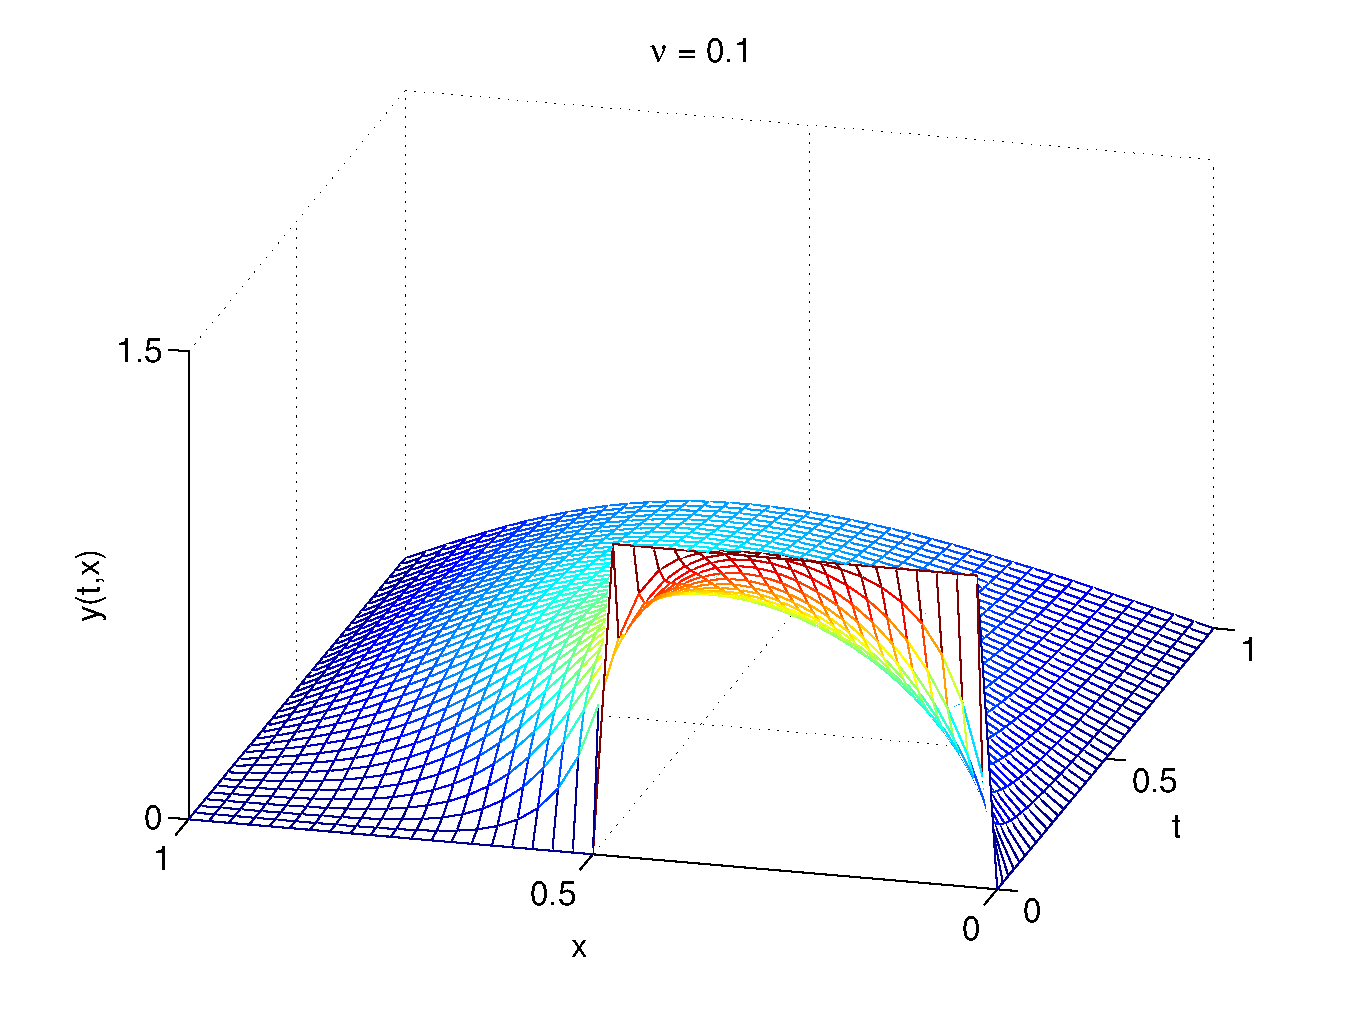
\includegraphics[width=0.33\textwidth]{plots/FullModel_nu01}}\hfill
\subfloat{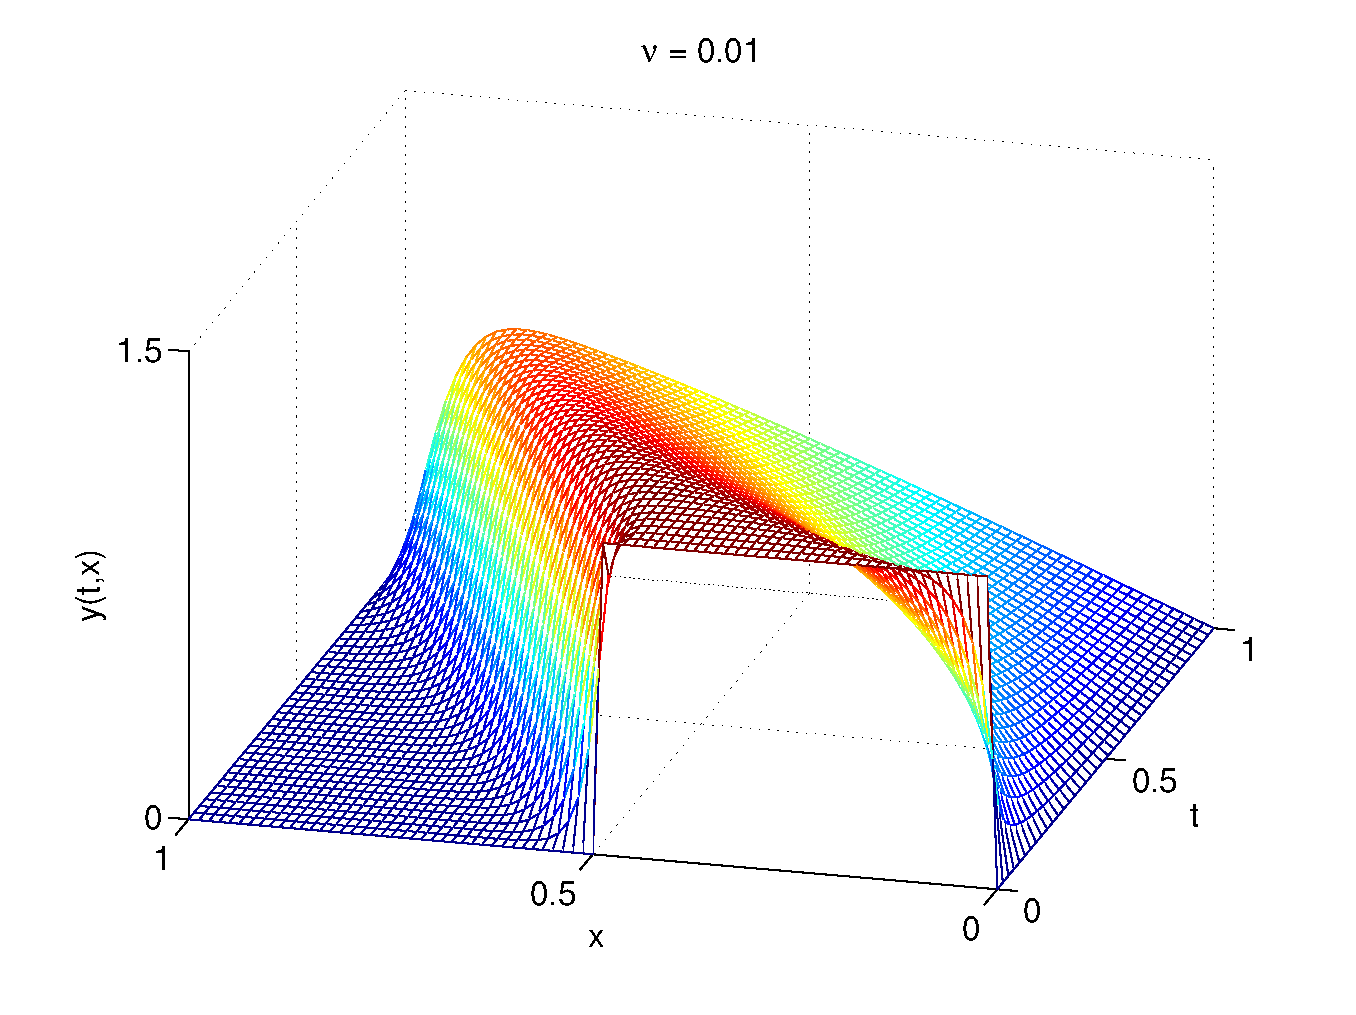
\includegraphics[width=0.33\textwidth]{plots/FullModel_nu001}}\hfill
\subfloat{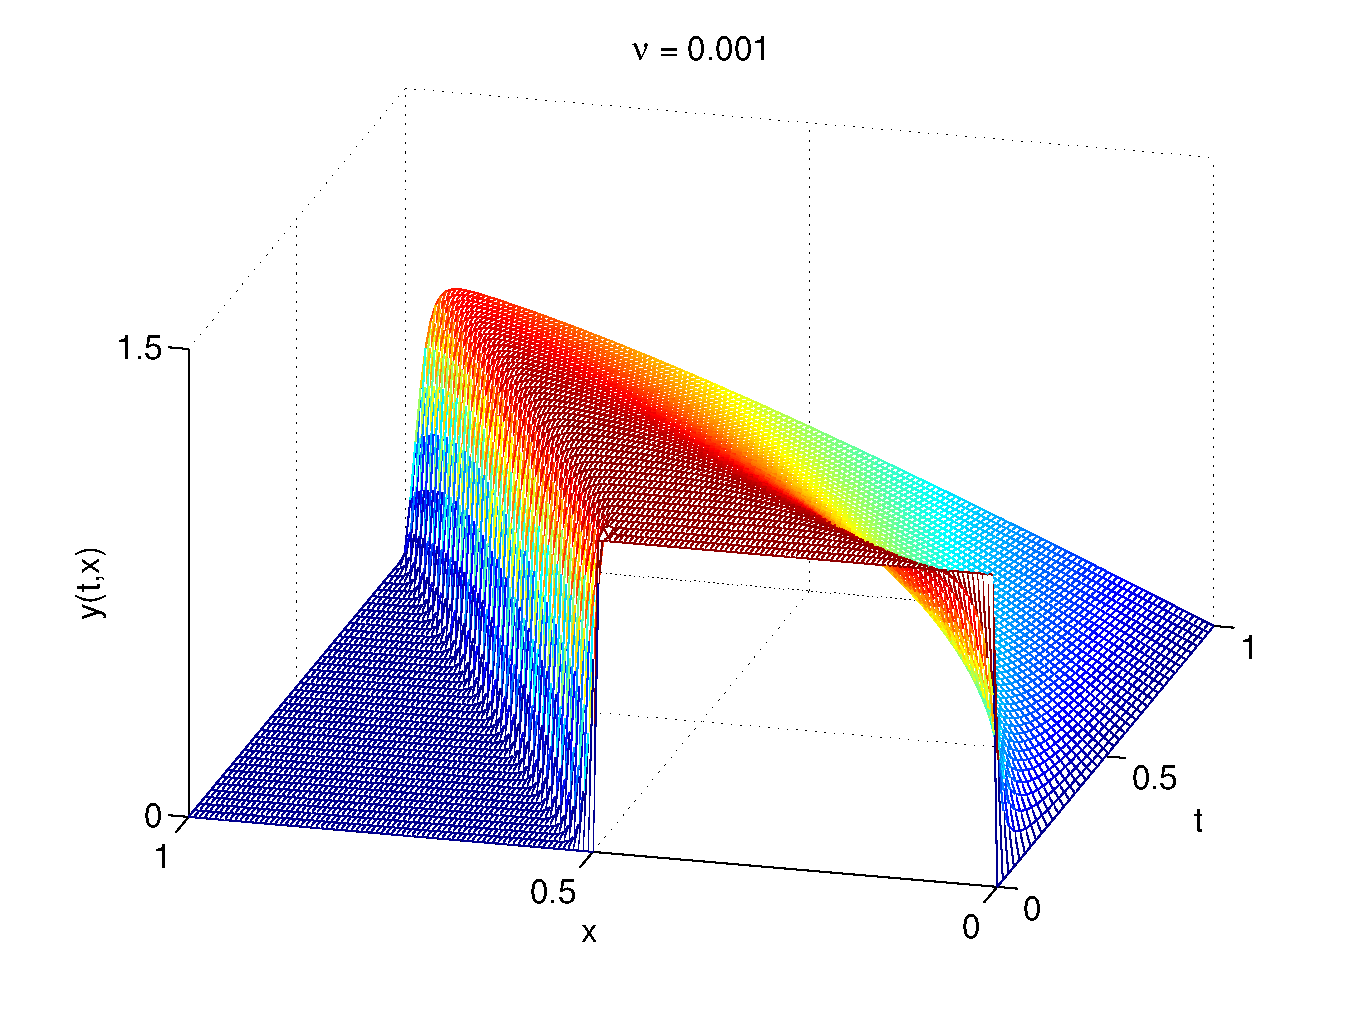
\includegraphics[width=0.33\textwidth]{plots/FullModel_nu0001}}\hfill
\caption{Numerical solution of the full-order Burgers' equation for different viscosity parameters $\nu = \{0.1, 0.01, 0.001\}$ and initial condition \eqref{FEMdiscr_init}.}\label{FullNumSol}
\end{figure}
According to \cite{KV99} the POD basis $\{\varphi_i\}_{i=1}^\ell$ can be obtained by solving the eigenvalue problem:
\begin{align}
\label{PODviaEW}
Y Y^T M \varphi = \sigma^2 \varphi,
\end{align}
where $Y$ is the matrix of snapshots as previously defined in \eqref{snapshots}, i.e. the columns of $Y$ are the solution of Burgers' equation at different time instances.

Since the mass matrix $M$ is symmetric and positive definite, there exists a Cholesky decomposition of the form $M = R^T R$. Multiplication of \eqref{PODviaEW} from the left with $R$ then yields,
\begin{align*}
R Y Y^T R^T R \varphi = \sigma^2 R \varphi,
\end{align*}
which is equal to
\begin{align}
\label{PODviaEW_final}
\bar{Y} \bar{Y}^T \bar{\varphi} = \sigma^2 \bar{\varphi},
\end{align}
for $\bar{Y} := RY$ and $\bar{\varphi} := R \varphi$. Because of the relation \eqref{SVDalsEW} between the SVD and eigenvalues, we can solve \eqref{PODviaEW_final} and, thus, also \eqref{PODviaEW} by the computation of an SVD of the matrix $\bar{Y} = RY$,
\begin{align}
\label{SVD_ss}
R Y = U \Sigma V^T.
\end{align}
After choosing a suitable POD dimension $\ell \ll N$, let us define the matrix of left singular vectors, $U_{\ell} := [u_1,...,u_{\ell}]$, where $u_i$ are the columns of the matrix $U$ in \eqref{SVD_ss}. Then, the POD basis is given by:
\begin{align}
\label{Phidef}
\Phi_{\ell} := R^{-1} U_{\ell},
\end{align}
and we denote the columns of $\Phi_\ell$ by $\varphi_i$ such that $\Phi_\ell = [\varphi_1,...,\varphi_\ell]$. The following ansatz leads to an approximation of the original full-order solution,
\begin{align}
\label{PODansatz}
\mathbf{y}(t) \approx \Phi_{\ell} \mathbf{\tilde y}(t) \quad \text{with } \mathbf{\tilde y}(t) \in \mathbb{R}^{\ell}.
\end{align}
The Galerkin projection of \eqref{FEMdiscr} onto $span \{\varphi_1,...,\varphi_\ell\}$ is given by
\begin{align}
\label{redSys}
\mathbf{\dot{\tilde y}}(t) = -\frac{1}{2} B_{\ell} (\Phi_{\ell} \mathbf{\tilde y}(t))^2 - \nu C_{\ell} \mathbf{\tilde y}(t),
\end{align}
with the matrices
\begin{align}
\label{Bl}
B_{\ell} &:= \Phi_{\ell}^T B \in \mathbb{R}^{\ell \times N},\\
\label{Cl}
C_{\ell} &:= \Phi_{\ell}^T C \Phi_{\ell} \in \mathbb{R}^{\ell \times \ell},
\end{align}
and with the new mass matrix equal to the $\ell \times \ell$ identity since:
\begin{align}
\label{Mortho}
M_{\ell} &:= \Phi_{\ell}^T M \Phi_{\ell} = U_{\ell}^T U_{\ell} = I_{\ell} \in \mathbb{R}^{\ell \times \ell}.
\end{align}
We will refer to \eqref{redSys} as the POD-reduced system. As shown in \eqref{Mortho}, due to the M-orthogonality of the projection matrix $\Phi_\ell$, the mass matrix in the POD-reduced system vanishes, and this leads to a simpler numerical treatment of \eqref{redSys} compared to the full-order system \eqref{FEMdiscr}. Note, that $\Phi_\ell \mathbf{\tilde y}(t) \in \mathbb{R}^N$ is still of large dimension and, therefore, no dimension reduction for the nonlinearity has been obtained so far. Also, the number of columns of the reduced matrix $B_\ell$ is still of large dimension $N$.

The projected initial condition for the original system is:
\begin{align*}
\Phi_{\ell} \mathbf{\tilde y}(0) &= \mathbf{y}(0), \\
R^{-1} U_{\ell} \mathbf{\tilde y}(0) &= \mathbf{y}(0),
\end{align*}
and, therefore, the initial condition for \eqref{redSys} can be obtained by pre-multiplication of the full-size initial condition with the matrix product $\Phi_{\ell}^T M$ as shown below:
\begin{align}
\label{initRed}
\mathbf{\tilde y}(0) &= U_{\ell}^T R \mathbf{y}(0) = \Phi_{\ell}^T R^T R \mathbf{y}(0) = \Phi_{\ell}^T M \mathbf{y}(0).
\end{align}
%Note that the initial condition of the full-order system is given in \eqref{FEMdiscr_init} and, thus, the respective initial condition of the reduced model follows directly from \eqref{initRed}.
%
As it has already been pointed out, the nonlinear term in \eqref{redSys} is still of large dimension $N$. We will now apply the DEIM method in order to reduce the computational complexity of evaluating the nonlinearity. Consider the snapshot matrix of the nonlinearity, \mbox{$F := [\mathbf{y}(t_1)^2,...,\mathbf{y}(t_{n_s})^2]$} and the corresponding Singular Value Decomposition:
\begin{align*}
 F = U_f \Sigma_f V_f^T.
\end{align*}
Again, by choosing the DEIM-dimension $m$, we are able to define the matrix of left singular vectors, $U_{m} := [u^f_1,...,u^f_{m}]^T$, which is used as an input basis for \mbox{Algorithm \ref{alg:DEIM}}. From \mbox{Algorithm \ref{alg:DEIM}}, we obtain the projection matrix $\mathcal{P}$ and the nonlinear term becomes:
\begin{align*}
 \Phi_{\ell}^T B (\Phi_{\ell} \mathbf{\tilde y})^2 = \Phi_{\ell}^T B U_{m} (\mathcal{P}^T U_{m})^{-1} \mathcal{P}^T (\Phi_{\ell} \mathbf{\tilde y})^2 \stackrel{(*)}{=} \underbrace{\Phi_{\ell}^T B U_{m} (\mathcal{P}^T U_{m})^{-1}}_{\ell \times m}(\underbrace{\mathcal{P}^T \Phi_{\ell}}_{m \times \ell} \mathbf{\tilde y})^2,
\end{align*}
where the step $(*)$ is allowed since squaring is a componentwise operation.
\newpage
\begin{figure}[H]
\centering
\subfloat{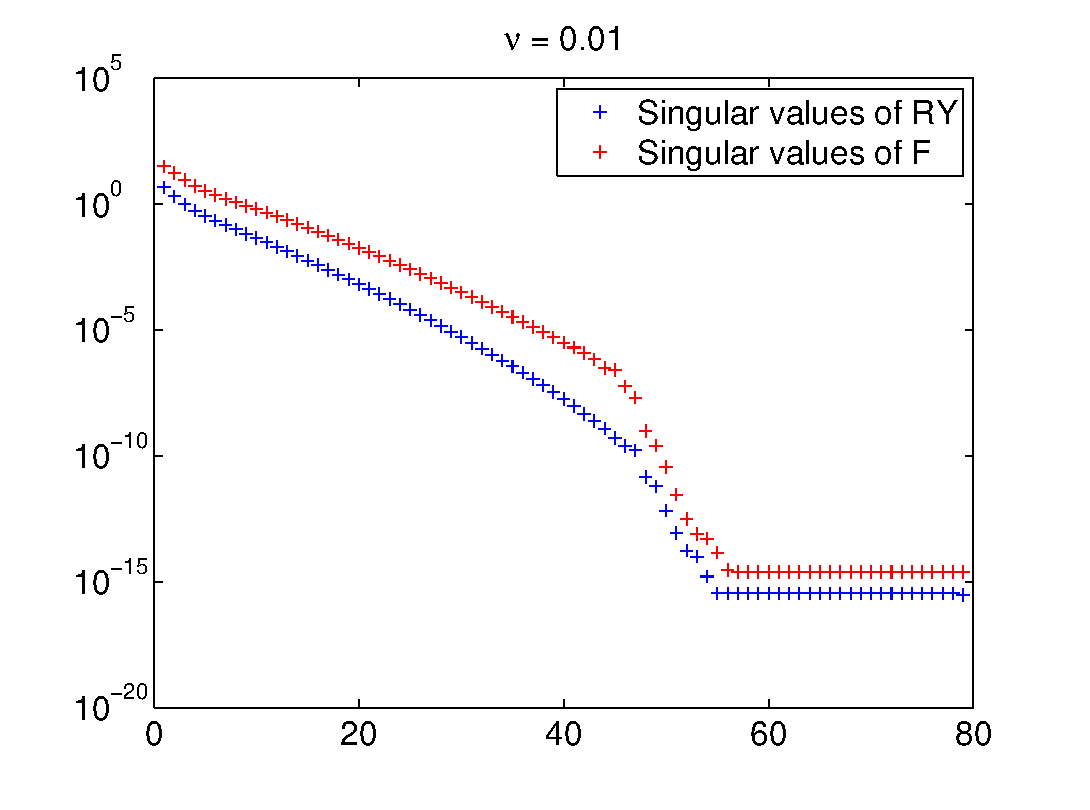
\includegraphics[width=0.49\textwidth]{plots/singValues_bignu}}\hfill
\subfloat{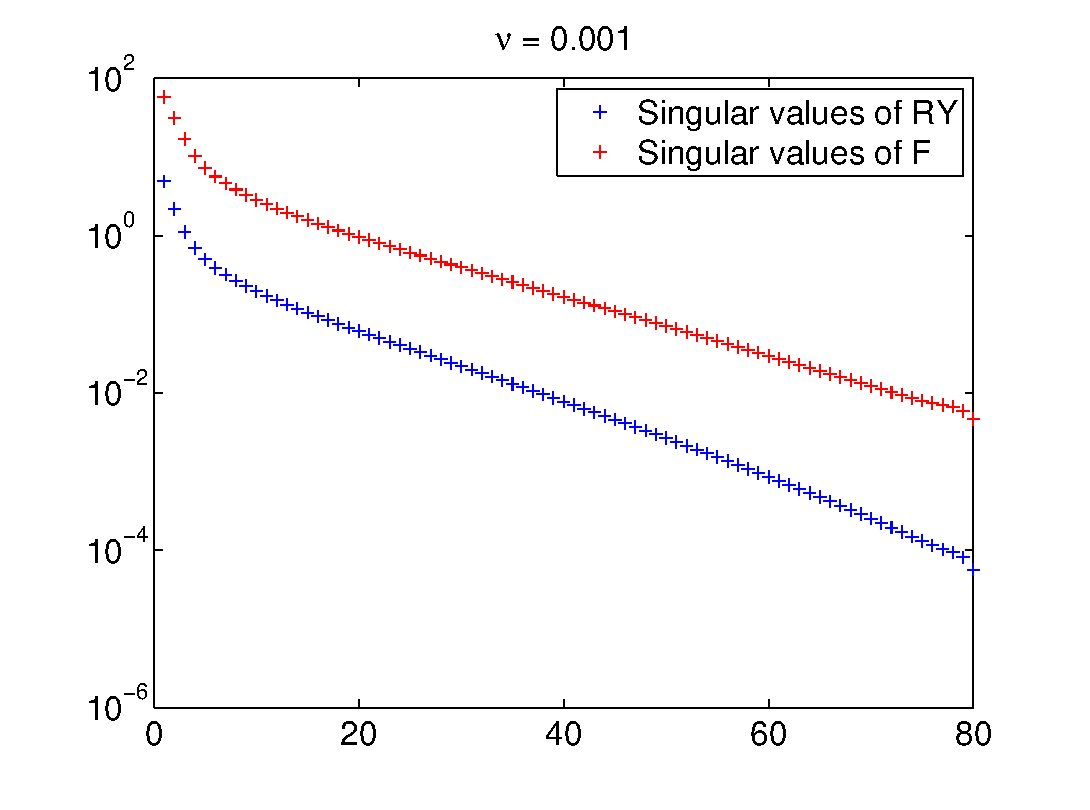
\includegraphics[width=0.49\textwidth]{plots/singValues_smallnu}}\hfill
\caption{Distribution of the singular values for $\nu = 0.01$ (left) and $\nu = 0.001$ (right).}\label{singVal}
\end{figure}
\noindent
The fully reduced POD-DEIM system is then given by
\begin{align}
\label{finalPODDEIM}
\mathbf{\dot{\tilde y}}(t) = -\frac{1}{2} \tilde B (\tilde F \mathbf{\tilde y}(t))^2 - \nu \tilde C \mathbf{\tilde y}(t) + \mathbf{\tilde f},
\end{align}
where
\begin{align}
\label{Bred}
\tilde{B} &:= \Phi_\ell^T B U_f(\mathcal{P}^T U_f)^{-1} \in \mathbb{R}^{\ell \times m},\\
\label{Cred}
\tilde{C} &:= \Phi_\ell^T C \Phi_\ell \in \mathbb{R}^{\ell \times \ell},\\
\label{Fred}
\tilde{F} &:= \mathcal{P}^T \Phi_\ell \in \mathbb{R}^{m \times \ell}.
\end{align}
Note that both matrices $\tilde{B}$ and $\tilde{F} $ can be pre-computed such that the system \eqref{finalPODDEIM} is indeed of dimension $\ell \times \ell$ and no dependence on the original \mbox{size $N$} exists anymore. As for the full-order system \eqref{FEMdiscr}, the POD-DEIM reduced system \eqref{finalPODDEIM} was solved by means of the implicit Euler method, see Appendix \ref{implEuler}. The choice of the dimensions of the reduced model $\ell$ and $m$ is crucial in order to obtain an accurate result of the reduced system that reproduces the dynamics of the original system. A good estimate for the choice of $\ell,m$ is given by the ration of the truncated sum of the singular values and the sum of all singular values given in \eqref{heuristics}. Therefore, we consider the distribution of the singular values of the respective snapshot matrices in Figure \ref{singVal}. We see that especially for $\nu = 0.01$, the first singular values decay tremendously which gives rise to a good approximation of the reduced system when only a small number for $\ell,m$ is chosen. We will present in Figure \ref{PODplot} the behavior of the numerical solution of the POD-DEIM reduced system when the DEIM-dimension $m$ is fixed and $\ell$ is increased.
\newpage
\begin{figure}[H]
  \centering
  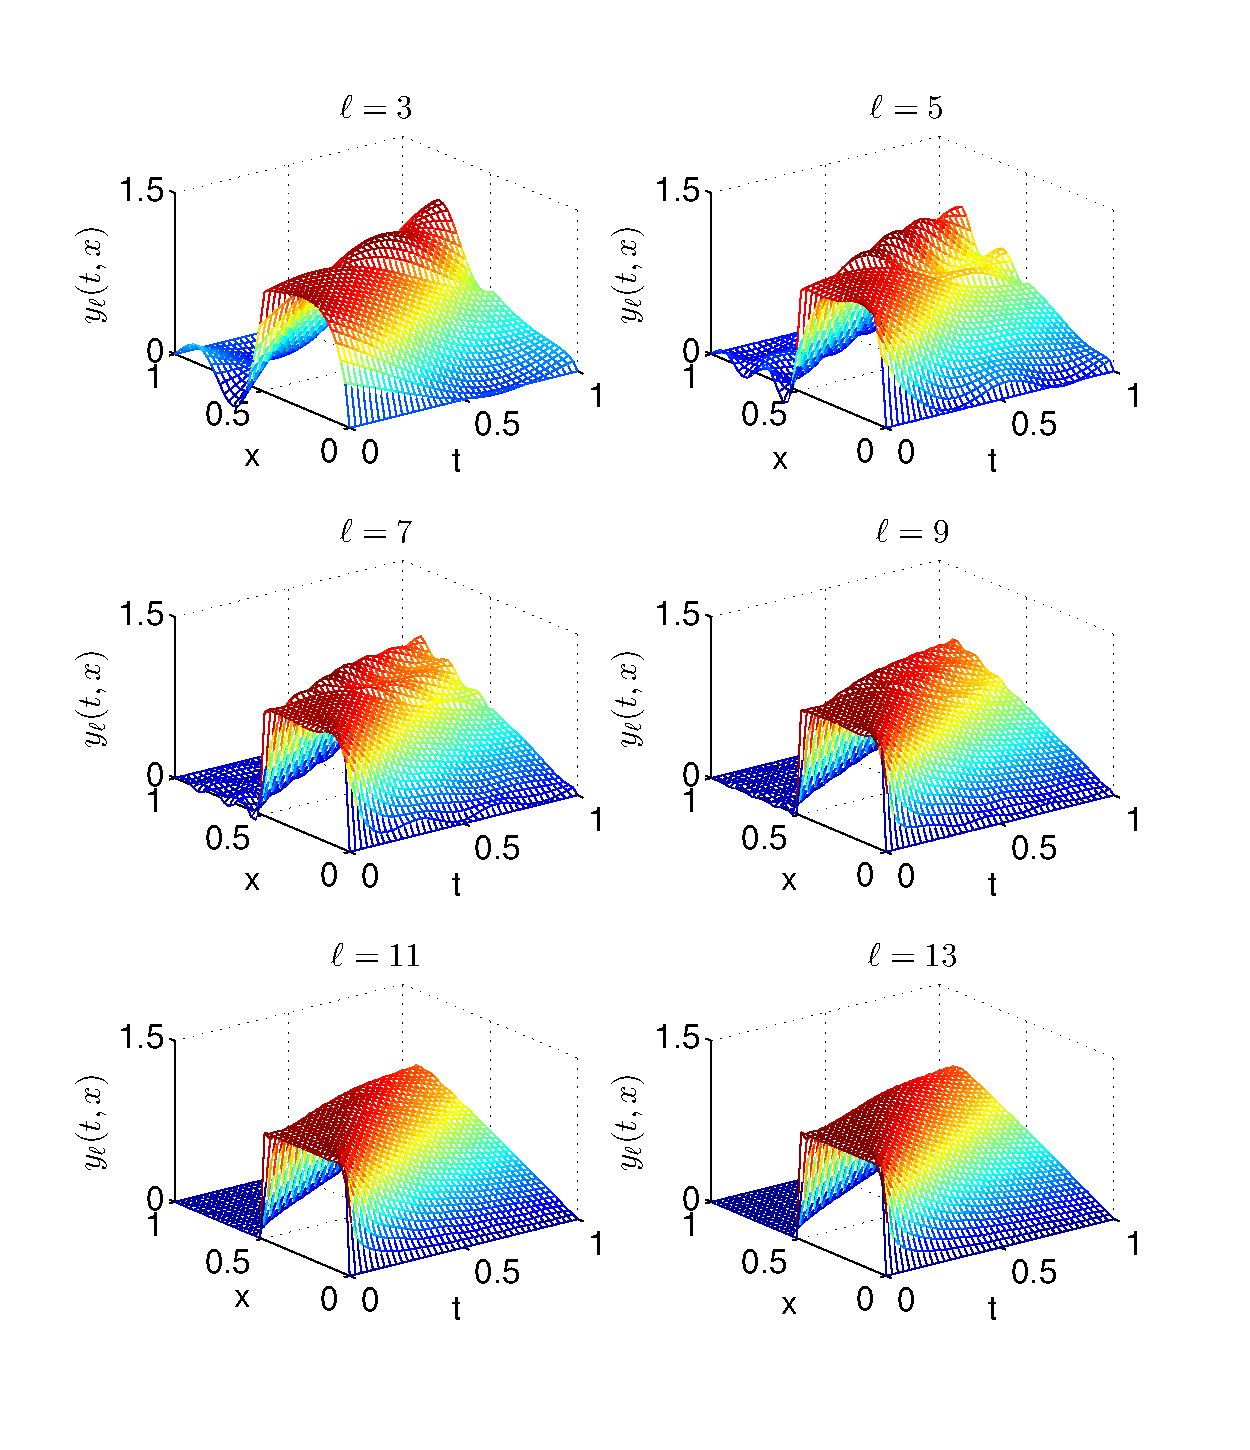
\includegraphics[width=\textwidth]{plots/PODplot_lnew.eps}\\
  \caption{POD-DEIM approximations for different dimensions $\ell$ and $m = 15$, $\nu = 0.01$.}\label{PODplot}
\end{figure}
Figure \ref{PODplot} shows the convergence of the POD-DEIM reduced model to the full-order solution. In each computation, a fixed DEIM dimension of $m = 15$ was used to approximate the nonlinear term in Burgers' equation. If the dimension of the POD basis $\ell$, i.e. the size of the projected model is increased, we see from Figure \ref{PODplot} that the numerical solution of the reduced system converges towards a smooth solution that corresponds to the solution of the original model.
\subsection{Approximation error}
We now focus on the accuracy of the approximated system's response computed with reduced models. Let $\mathbf{y}$ be the response of the full-order system, $\mathbf{y}^{(\ell)} = \Phi_\ell \mathbf{\tilde y}$ be the response of the POD-reduced model \eqref{redSys} obtained with a POD basis of dimension $\ell$, and let $\mathbf{y}^{(\ell,m)} = \Phi_\ell \mathbf{\tilde y}$ be the response of a reduced model obtained with POD-DEIM \eqref{finalPODDEIM}, with a POD basis is of dimension $\ell$ and a DEIM basis of dimension $m$. Then, we define the $L_2(\Omega)$ relative error in an approximate response $\mathbf{\bar{y}}$ with respect to the full-order-system's response $\mathbf{y}$ as:
\begin{align}
\label{relErr_def}
\bar{e} := \frac{\|\mathbf{y} - \mathbf{\bar{y}}\|_{L_2(\Omega)}}{\|\mathbf{y}\|_{L_2(\Omega)}} \approx \frac{\sqrt{h \cdot \delta \! t \cdot \sum_{i,j} [y_i(t_j) - \bar{y}_i(t_j)]^2}}{\sqrt{h \cdot \delta \! t \cdot \sum_{i,j} y_i^2(t_j)}},
\end{align}
where $\Omega = [0,L] \times [0,T]$, and $h$ and $\delta \! t$ are the step size in space and time, respectively. In our test cases, we have chosen $T = L = 1$ and, hence, $\Omega = [0,1] \times [0,1]$. The approximate response $\mathbf{\bar{y}}$ in \eqref{relErr_def} is  $\mathbf{\bar{y}} = \mathbf{y}^{(\ell)}$ for POD and $\mathbf{\bar{y}} = \mathbf{y}^{(\ell,m)}$ for POD-DEIM.

%In order to show the convergence of the reduced POD-DEIM model to the full-order system in more detail, we computed both, the numerical solution of the full-order system $\mathbf{y}$ as well as the numerical solution of the reduced-order model which we denote by $\mathbf{y}^{(\ell,m)}$. By the superscript we mean that $\mathbf{y}^{(\ell,m)}(t) = \Phi_\ell \mathbf{\tilde y}(t)$, where the reduced variable $\mathbf{\tilde y}$ has been obtained by the POD-DEIM reduced model \eqref{finalPODDEIM} with POD dimension $\ell$ and DEIM-dimension $m$, respectively. For $\Omega = [0,L] \times [0,T]$, with $L = T = 1$, we define the relative error $e_{\ell}$ using an approximation of the $L_2(\Omega)$ norm as:
%\begin{align}
%\label{relErr_def}
%e_{\ell,m} := \frac{\|\mathbf{y} - \mathbf{y}^{(\ell,m)}\|_{L_2(\Omega)}}{\|\mathbf{y}\|_{L_2(\Omega)}} \approx \frac{\sqrt{h \cdot \Delta t \cdot \sum_{i,j} [\mathbf{y}_i(t_j) - \mathbf{y}^{(\ell,m)}_i(t_j)]^2}}{\sqrt{h \cdot \Delta t \cdot \sum_{i,j} \mathbf{y}_i^2(t_j)}},
%\end{align}
%where $h$ and $\Delta t$ are the step size in space and time, respectively. In the same way, we denote by $e_\ell$ the relative error that compares the full-order solution with an approximation obtained by the POD-reduced system \eqref{redSys} with the POD dimension equal to $\ell$.
In Figure \ref{relErr}, show the behavior of the relative error when either the DEIM-dimension is fixed (left) or the POD dimension is fixed (right). From the numerical results that have been obtained for a viscosity parameter $\nu = 0.01$ and a full-order dimension of $N = 80$, we observe that the error of the POD and the POD-DEIM reduced model are of the same magnitude until the POD dimension exceeds the DEIM-dimension which has been fixed in the left plot to $m = 15$. When $\ell$ is larger than $m$ in the left plot, we observe that only the POD-reduced model is still improved while the error of the POD-DEIM reduced model seems to be dominated by the error caused by the DEIM approximation of size $m = 15$. %Figure \ref{relErr} shows the behavior of the relative error as the POD dimension $\ell$ increases. We see from the plot that from $\ell = 11$ on, the relative error is of the order $\mathcal{O}(10^{-4})$. Since the full-order system consists of $N=50$ grid points in space, we conclude that in this specify setup the reduced order model of approximately one fifth of the size of the original system already leads to results of a very good accuracy.
\begin{figure}[H]
  \centering
  \subfloat{\includegraphics[width=0.49\textwidth]{plots/rel_Err_newleft_NEW}}\hfill
  \subfloat{\includegraphics[width=0.49\textwidth]{plots/rel_Err_newright_NEW}}\hfill
  \caption{Relative error of the POD and POD-DEIM approximation for a fixed number of DEIM basis $m = 15$ (left) and a fixed number of POD basis $\ell = 15$ (right).}\label{relErr}
\end{figure}
The right plot in Figure \ref{relErr} shows the same behavior, i.e. an increase of the DEIM-dimension does not lead to a better approximation once it is larger than a given POD basis dimension. In Figure \ref{relErrml}, we observe this behavior for all combinations of $(\ell,m)$ in a range of \texttt{3:2:39}. These observations seem to indicate that for optimal dimension reduction using the POD-DEIM approach, we need to choose $\ell$ and $m$ in such a way that they are almost of the same size.
\begin{figure}[H]
  \centering
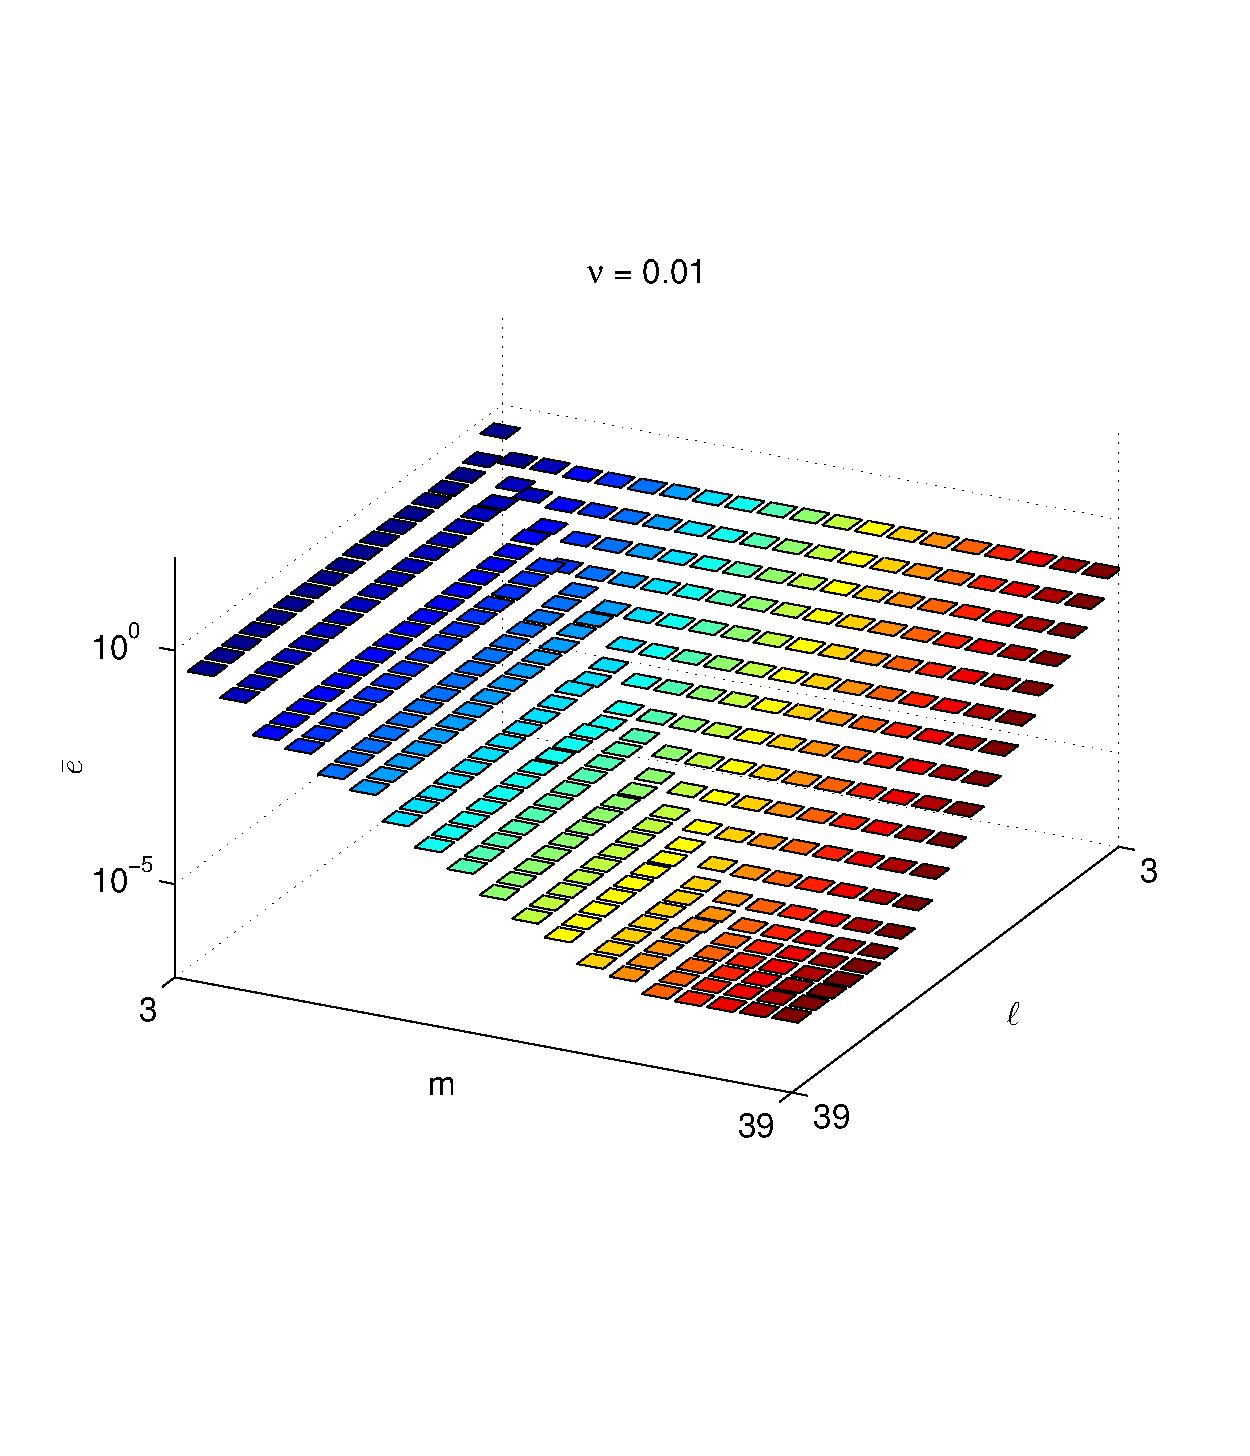
\includegraphics[width=0.7\textwidth]{plots/err_lm_NEW}
  \caption{Relative error of the POD-DEIM reduced model as a function of the reduced-model dimensions $\ell$ and $m$.}\label{relErrml}
\end{figure}

\subsection{Use of POD-DEIM for parameter studies}
In \cite{CS10}, the authors propose to use POD-DEIM also for parameter studies of a given dynamical system. In the case of Burgers' equation, this means that we simulate the full-order system twice for two different values of the viscosity parameters $\nu_{left} = 0.001$ and $\nu_{right} = 0.1$, using $N=400$ grid points in space which is necessary when dealing with very small values for $\nu$. The numerical solutions of the full-order system for both viscosity parameters were presented in Figure \ref{FullNumSol} where we can observe that the value of the viscosity parameter plays a crucial role in the propagation of the initial impulse in time. For large $\nu$, the solution becomes much more diffusive and, therefore, the initial condition vanishes very fast. For small $\nu$, the initial condition is propagated in time almost without losing height.
%\begin{figure}[H]
%\includegraphics[width=0.99\textwidth]{plots/param_study_both}
%\caption{Full-order system for $\nu=0.001$ (left) and $\nu = 0.1$ (right).}\label{param_study_both}
%\end{figure}
The benefit of POD-DEIM for parameter studies is that a reduced model can be obtained for any parameter $\nu$ that lies within the interval $[\nu_{left},\nu_{right}]$ only from data of the full-order model corresponding to $\nu_{left}$ and $\nu_{right}$. Suppose we are interested in an approximation of the numerical solution for $100$ different viscosity parameter in $[\nu_{left},\nu_{right}]$, we only need to solve the full-order system twice and are able to obtain a reduced model from these data.

The reduction is based on a singular value decomposition of the combined matrices
\begin{align*}
Y = [Y_{\ell} | Y_{r}], \quad F = [F_{\ell} | F_{r}],
\end{align*}
where $Y_{\ell}$ and $F_{\ell}$ are snapshot matrices of the solution and the nonlinearity corresponding to $\nu_{left}$ and $Y_{r}$ and $F_r$ correspond to $\nu_{right}$, respectively. The POD basis is then derived using the snapshot matrix $Y$ that contains information of the dynamical behavior of Burgers' equation with viscosity parameter $\nu_{left}$ and $\nu_{right}$. Similarly, the DEIM projection matrix $\mathcal{P}$ is obtained from the matrix $F$.

In Figure \ref{param_study_inner}, the POD-DEIM approximation for the viscosity parameter $\nu = 0.01$ using the dimensions $\ell = m = 45$ is presented as well as the full-order model of dimension $N = 400$ for the same viscosity parameter. The plot shows the good quality of the reduced system. At this point, we want to stress that in order to obtain the POD-DEIM model in Figure \ref{param_study_inner}, the simulation of the full-order system with parameter $\nu = 0.01$  was not taken into account. Therefore, the derivation of a reduced model for any parameter $\nu \in [\nu_{left}, \nu_{right}]$ only requires the computational work of the numerical solution of the reduced system once the matrices $Y$ and $F$ are obtained.
\begin{figure}[H]
\includegraphics[width=0.99\textwidth]{plots/param_study_inner}
\caption{Response of the full-order system and of the POD-DEIM reduced model for $\nu=0.01$.}\label{param_study_inner}
\end{figure}
\subsection{Computational speedup for POD and POD-DEIM}
\label{sect2_numTests}
In the previous chapters, the main focus lies on the size of the reduced system and the quality of the approximation compared to the full-order system. In this section, we are interested in the speedup of the computation when POD or POD-DEIM is applied. Therefore, we consider the numerical solution of Burgers' equation as described in Appendix \ref{FEMDiscr} for different viscosity parameters $\nu$. From the numerical analysis of the full model, it is well-known that for different sizes of $\nu$ a different size of the spatial discretization is required in order to obtain a stable numerical solution. In \ref{Tab2}, we have chosen the smallest value of $N$ for which the full-order solution is stable.

The following quantities have been measured during the numerical simulation:
\begin{itemize}
  \item $t_{setup}$ - The time which is required to pre-compute the matrices \eqref{Bl}, \eqref{Cl} in the case of pure POD and \eqref{Bred}-\eqref{Fred} in the case of POD-DEIM. Note that this only has to be performed once.
  \item $t_{PDEsol}$  - The time for the numerical solution of Burgers' equation. This has been done via the implicit Euler method and a Newton iteration for the time integration and a finite elements approach for the spatial discretization.
  \item $\bar{e}[10^{-4}]$  - The relative error in $L_2([0,1] \times [0,1])$ as defined in \eqref{relErr_def}.
  \item $S_P^{(1)}$  - The overall speedup which is defined as the ratio of the computational time for the full-order model and the respective reduced model.
  \item $S_P^{(2)}$ - The speedup when only the numerical solution of Burgers' equation is taken into account. Here, we neglect the time that is required for the pre-computation in $t_{setup}$.
\end{itemize}

In order to obtain comparable results, we decided to choose the reduced dimensions $\ell$ and $m$ such that the relative error $\bar{e}$ in the response of each of the reduced models has the same order of magnitude, $\bar{e} \in \mathcal{O}(10^{-4})$. Therefore, we indicate in the first row of \mbox{Table \ref{Tab2}} the important dimension from the respective model. In case of the full-order model, we present the number $N$ of ansatz function of the FEM discretization. For the pure POD reduced model we give the size of the POD basis, $\ell$, and for the the POD-DEIM reduced model we present the dimensions as a tuple $(\ell,m)$.
\begin{table}[H]
\centering
\begin{tabular}{|c|c|c|c|c|c|c|c|c|c|}
\cline{1-10}
 & \multicolumn{3}{ c| }{$\nu = 0.01$} & \multicolumn{3}{ c| }{$\nu = 0.001$}& \multicolumn{3}{ c| }{$\nu = 0.0001$}\\ \cline{2-10}
 & Full & POD & DEIM & Full & POD & DEIM & Full & POD & DEIM \\ \cline{1-10}
$N$/$\ell$/$m$ & $80$ &$ 11 $&$(11,13)$ & $200$&$35 $& $(35,40)$  & $800$&$40 $& $(40,55)$ \\ \cline{1-10}
$t_{setup}[s]$        & -      &0.003      &0.011       & -    &0.009&0.021 & -& 0.0729&0.182\\ \cline{1-10}
$t_{PDEsol}[s]$   &  0.068     &0.047      &0.040       & 0.232&0.12&0.055 & 4.416&0.276&0.085\\ \cline{1-10}
$\bar{e}[10^{-4}]$   & -      &6.13       &6.46        & -    &6.12&6.85 & -&7.43& 7.66\\ \cline{1-10}
$S_P^{(1)}$           & -      &1.35       &1.34        & -    &1.74&3.03 & -&12.54&16.52\\ \cline{1-10}
$S_P^{(2)}$           & -      &1.44       &1.71        & -    &1.88&4.21 & -&15.85&51.85\\ \cline{1-10}
\end{tabular}
\caption{Comparison between POD and POD-DEIM for different values of $\nu$.} \label{Tab2}
\end{table}
We first note that for all different sizes of the viscosity parameter $\nu \in \{0.01, 0.001, 0.0001\}$ it is in general possible to derive a POD and POD-DEIM reduced model of a tremendously smaller dimension and a high accuracy of $\bar{e} \in \mathcal{O}(10^{-4})$. The numerical tests of Table \ref{Tab2} are presented in order to illustrate two features of the POD-DEIM approach. Firstly, we see that the time which is required for the numerical solution of the POD-DEIM reduced model does not increase when the size of the original problem, $N$, increases. On the other hand, we see that the solution of the pure POD model still depends on the original problem size and increases with $N$. This behavior is illustrated in Figure \ref{depN} where we see that the increase in $N$ only affects the computation time of the POD model. Its independence of the original (large) dimension is the reason for the large speedup obtained when using the POD-DEIM reduced model. We see that for $N=3,000$, the POD-DEIM model is almost five times faster than the pure POD model. Secondly, we observe that in order to apply DEIM, it is more costly to apply the required pre-computations of the matrices \eqref{Bred}-\eqref{Fred}. This is mostly because two singular value decompositions are required in order to obtain the projection basis and the input basis for the DEIM Algorithm \ref{alg:DEIM}. This is also the reason why the overall speedup $S_P^{(1)}$ of POD and POD-DEIM for the presented test configurations is comparable even though DEIM leads to a higher speedup. The most important observation from the results in Table \ref{Tab2} is, however, that for the case $\nu = 0.0001$ and $N = 800$, we are able to show a speedup of the POD-DEIM method of more than $50$ compared to the full model while POD only leads to a speedup of $\sim \! 16$. This speedup computation only takes into account the time that is required to actually solve the reduced system numerically. Therefore, we conclude that DEIM leads to a tremendous reduction in computational cost as long as we are able to pre-compute the matrices \eqref{Bred}-\eqref{Fred} only once and then solve the reduced system many times. This conclusion gives rise to the application of POD-DEIM within an optimization iteration as described in the Chapter \ref{Opt_chap}.
\begin{figure}[H]
\centering
\subfloat{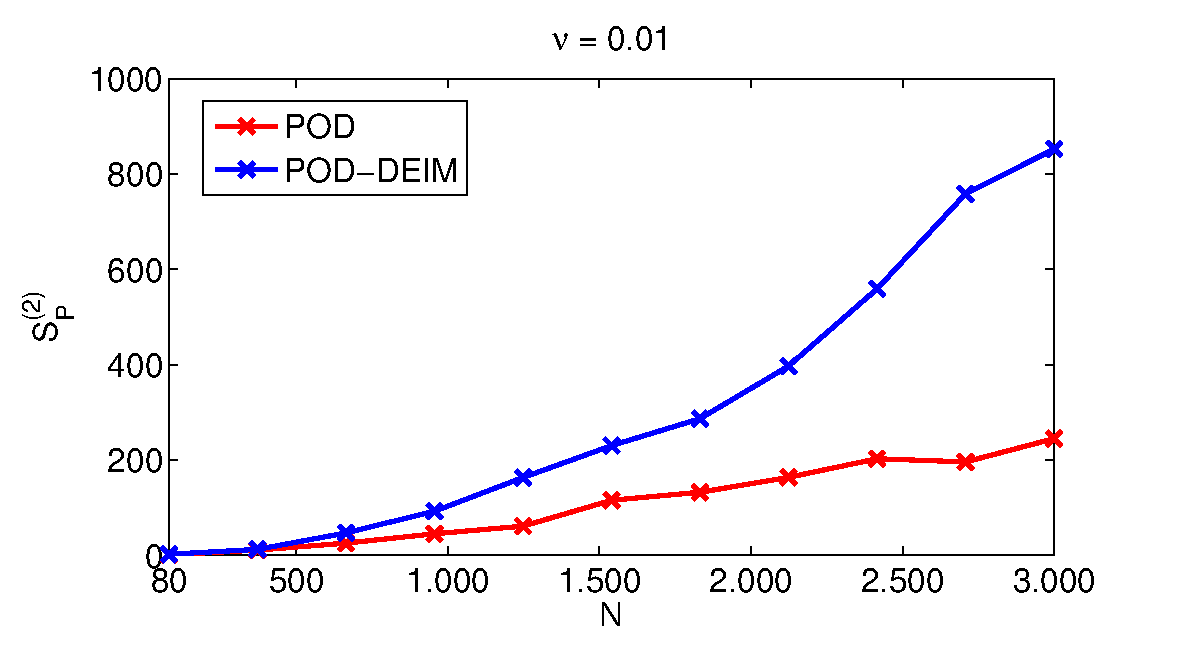
\includegraphics[width=0.49\textwidth]{plots/PODDEIM_Sp2}}\hfill
\subfloat{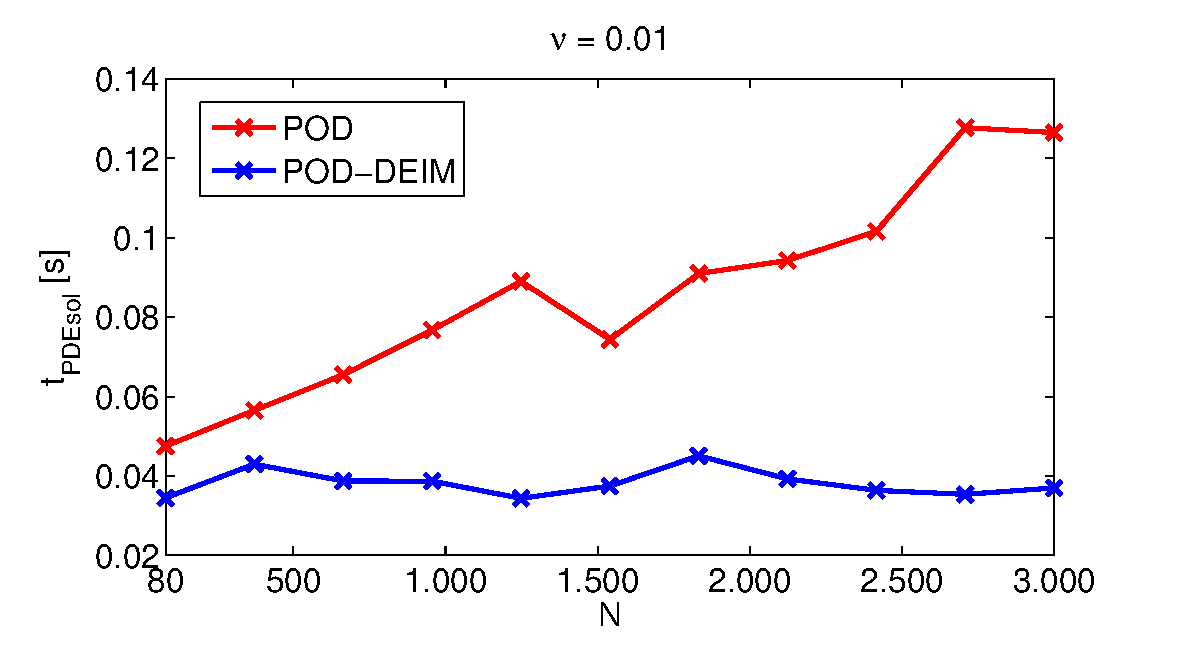
\includegraphics[width=0.49\textwidth]{plots/PODDEIM_Tsol}}\hfill
\caption{Dependence of the reduced models on the full-order dimension $N$.}\label{depN}
\end{figure}

%In the previous chapters, the main focus lies on the size of the reduced system and the quality of the approximation compared to the full-order system. In this section, we are interested in the speed-up of the computation when POD and POD-DEIM is applied. Therefore, we consider Burger's equation with viscosity parameter $\nu = 0.003$ on a spatial domain $[0,1]$ and end time $T = 4$. This requires a spatial and time discretization of $N = N_t =400$ points in order to obtain a stable numerical simulation. The reduced model with dimensions $\ell=m=45$ leads to an approximation of high accuracy (see Table \ref{Tab1}).
%
%The following quantities have been measured during the numerical simulation:
%\begin{itemize}
%  \item $t_s$ - The time which is required to pre-compute the matrices \eqref{Bl}, \eqref{Cl} in the case of pure POD and \eqref{Cl}, \eqref{Bred}, \eqref{Fred} in the case of POD-DEIM.
%  \item $t_{Eul}$ - The time for the time integration via the implicit Euler method and Newton's iteration.
%  \item $\bar e$ - The relative error in $L_2([0,1] \times [0,4])$.
%  \item $S_P$ - The overall speed-up which is defined as the ratio of the computational time for the full-order model and the reduced model.
%\end{itemize}
%In Table \ref{Tab1}, the speed-up of pure POD and POD-DEIM are compared: The application of POD of dimension $\ell = 45$ leads to a speed-up of the computation of approximately $3.5$ times the time of the original-size solution. If in addition DEIM is applied with dimension $m = 45$, we notice that the speed-up compared to the full-order model is $11.6$ which is approximately a speed-up of another $3.5$ times compared to the pure POD method. Therefore, in this setting the computational benefit of POD and POD-DEIM is almost of the same size. Note that both dimensions have been chosen in such a way that the relative error is of the order $\mathcal{O}(10^{-4})$ in both cases and, thus, the accuracy of the approximations is comparable for both cases.
%\begin{table}[H]
%\centering
%\begin{tabular}{l|c|c|c}
%& Full Order Model & POD & POD-DEIM \\
%\hline
%$t_s$ & - &  0.0018s& 0.0021s\\
%$t_{Eul}$ & 18.0785s& 5.1342s & 1.5189s\\
%$\bar e$ & - & 1.2805e-04 & 2.5057e-04\\
%$S_P$ & - &  3.5199 & 11.6801 \\
%\end{tabular}
%\caption{Comparison between POD and POD-DEIM for $\nu = 0.003$.} \label{Tab1}
%\end{table}
